\documentclass{report}
\usepackage[utf8]{inputenc}
\usepackage{amsmath, amsfonts, amsthm, graphicx, lipsum}
\usepackage{hyperref}
\hypersetup{
    colorlinks=true,
    linkcolor=blue,
    urlcolor=red,
    pdftitle={Tarea 5},
    }
\usepackage[margin = 1 in]{geometry}

\usepackage{fancyvrb}
\usepackage{fancyhdr, lastpage}
\pagestyle{fancy}
\lhead{Tarea 5: Algoritmo Floyd Warshall}
\rhead{Universidad Autónoma de Nuevo León}
\cfoot{Page \thepage\ of \pageref{LastPage}}

\usepackage{etoolbox} %Use carefully!
\patchcmd{\chapter}{\thispagestyle{plain}}{\thispagestyle{fancy}}{}{}

\usepackage[Glenn]{fncychap}
%Options: Sonny, Lenny, Glenn, Conny, Rejne, Bjarne, Bjornstrup
\usepackage{xcolor}
\usepackage{tikz}
\usepackage[most]{tcolorbox}

\newtcbtheorem{theo}%
  {Theorem}{}{theorem}
  
\usepackage{siunitx}
\usepackage{setspace}
\onehalfspacing

%-----------------------------------------------------------------------------------------------------------------
%   Nuevos Comandos
%-----------------------------------------------------------------------------------------------------------------
\newcommand{\war}{ \textit{{\bfseries{Floyd Warshall}}} }

\begin{document}

\section*{Algoritmo \war}

El código se baso en algoritmo \war enunciado en clase, se utilizaron diccionarios para representar los arcos, para después recopilar una matriz de estos mismos.

Se tomaron 3 ejemplos para correr el código. El código permite leer los valores de la matriz de adyacencia a través de un archivo .txt, de igual manera se pueden insertar de manera manual en los archivos .txt.

Los resultados se imprime en la pantalla pero se puede activar la función para guardarlos en un archivo de resultados.

De igual manera se pueden generar matrices adyacentes aleatorias de grafos no dirigidos en el archivo de jupyter python notebook.

Por último al momento de ejecutarlo nos pide los nodos de inicio y final para reportarnos el total de la ruta corta, y su camino.

\section*{Grafos}

Los grafos utilizados fueron los sguientes:

\begin{figure}[h!]
  \begin{minipage}[b]{0.4\linewidth}
  \centering
  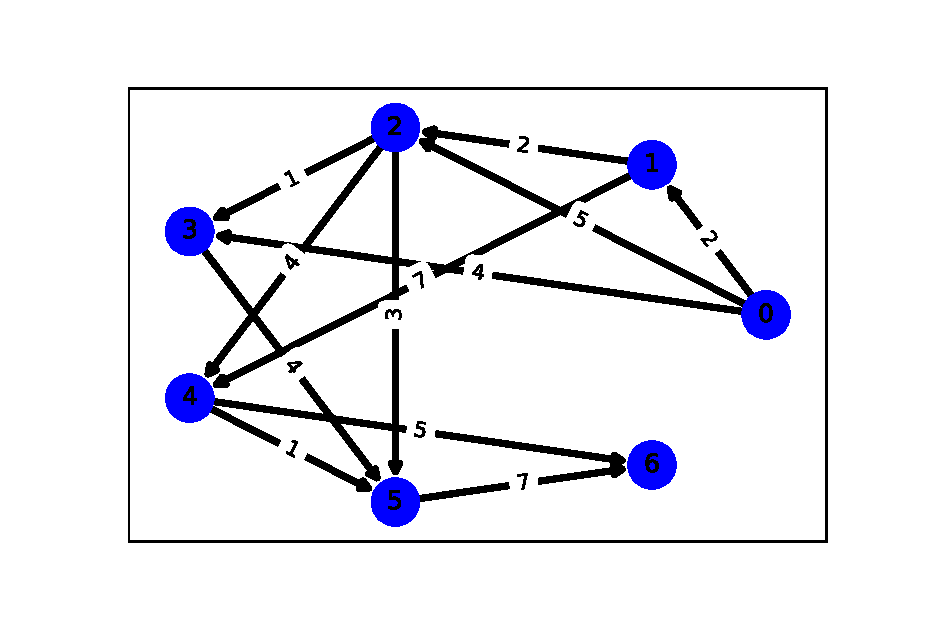
\includegraphics[width=\linewidth]{ejemplo1.eps}
  \caption{Grafo 1}
  \end{minipage}
  \hspace{0.5cm}
  \begin{minipage}[b]{0.5\linewidth}
  \centering
  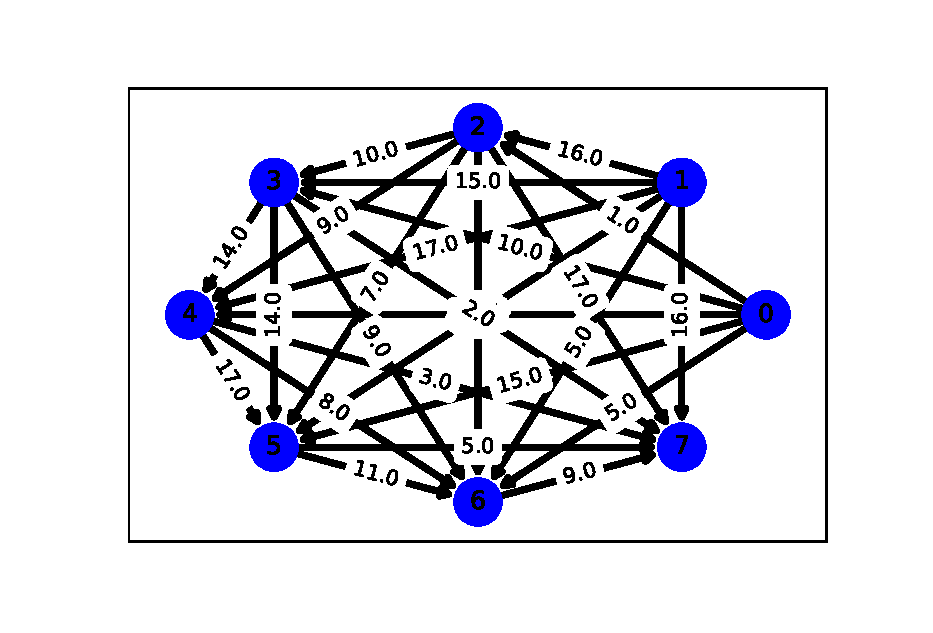
\includegraphics[width=\linewidth]{ejemplo2.eps}
  \caption{Grafo 2}
  \end{minipage}
\end{figure} 

\begin{figure}[h!]
\centering
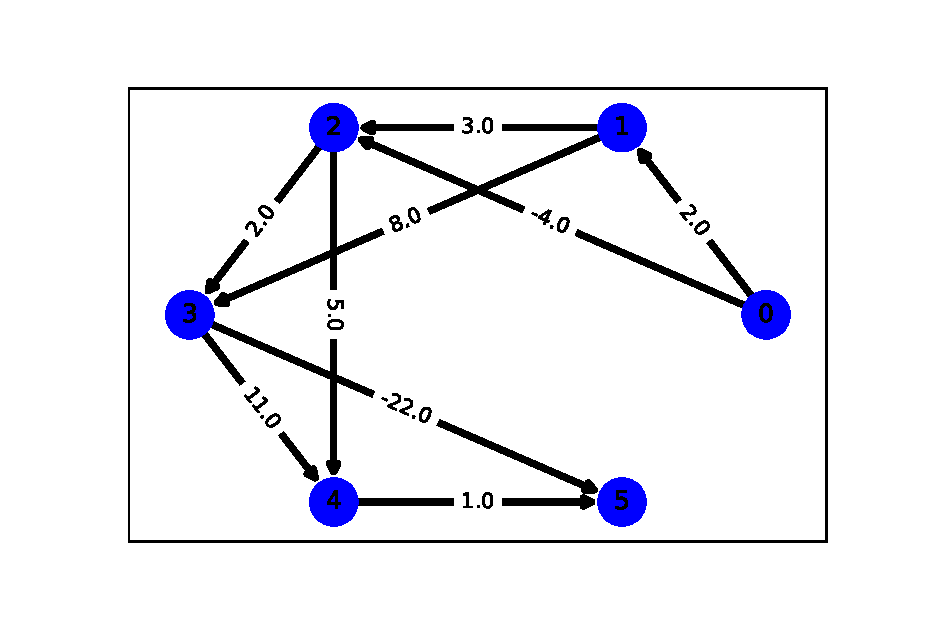
\includegraphics[scale = 0.5]{ejemplo3.eps}
\caption{Grafo 3}
\end{figure}

\newpage
Los resultados son los siguientes: 

\begin{minipage}[b]{0.3\linewidth}

En la Figura 1 los resulados  son los siguientes:

El costo menor es de 13

El camino es de: 

0 1 2 4 6 
  \end{minipage}
  \hspace{0.5cm}
\begin{minipage}[b]{0.3\linewidth}
En la Figura 2 los resulados  son los siguientes:


  El costo menor es de -1

El camino es de: 

0 2 5 7 
\end{minipage}
\hspace{0.5cm}
\begin{minipage}[b]{0.3\linewidth}
En la Figura 3 los  resulados  son los siguientes:

  El grafo tiene un ciclo  negativo 

El costo menor es de inf 

El camino es de: 

0 5 
  \end{minipage}







\end{document}